\documentclass[11pt, a4paper]{article}

\usepackage{amsmath}
\usepackage{amsfonts} %Matheschriften
\usepackage{amssymb} %Mathesymbole
%\usepackage{mathptmx} % Einstellung für Schriften und Sonderzeichen in mathematischen Umgebungen
                        % ändert SChriftfont
\usepackage{wasysym} % Stellt diverse Sonderzeichen bereit
\usepackage{siunitx}
\usepackage{float}
\usepackage{microtype}
\usepackage{graphicx}
\usepackage{hyperref}
\usepackage{xcolor}
\usepackage[section]{placeins}
% allows for temporary adjustment of side margins
\usepackage{changepage}
\usepackage{rotating}
\usepackage{physics}

\usepackage[ngerman]{babel}
\addto\captionsngerman{%
 \renewcommand{\abstractname}{Einleitung}}


\title{Versuch 3: Optischeabbildungen}
\author{Team 4-11: Jascha Fricker, Benedict Brouwer}

\begin{document}
    \maketitle

    \tableofcontents

    \newpage

    \section{Theorie}
    \FloatBarrier
    In der Physik spielen Linsen in optischen Versuchsuafbauten eine sehr wichtige Rolle. In diesem Versuch soll es darum gehen, verschiedene 
    Methoden auszuprobieren um den Brechungsindex und Hauptebenenabstand verschiedener Lisnen bzw Linsensysteme zu messen.
    \subsection{Autokollimation}
    Wie in Abbildung \ref{fig:autoKollAbb} zu sehen ist, wird die zu untersuchende Linse zwischen Blende und Spiegel gestellt. Nun wird der Abstande $l$ zwischen 
    Linse und Blende so eingestellt, dass auf der Blende welche gleichzeitig als Schirm dient ein Scharfes Bild entsteht. Dieser Vorgang wird wiederholt mit der um $180^\circ$ gedrehten Linse und der Abstand $k$ gemessen.
    Aus diesen Daten lassen Sich Brechungsindex und Hauptebenenabstand wie folgt berechnen:

    \begin{align}
    
    f' = \frac{k+l-h}{2} \label{eq:autokollBrech}\\
    h = k + l - 2 \cdot f' \label{eq:autokollHaupt}
        
    \end{align}

    \begin{figure}
        \centering
        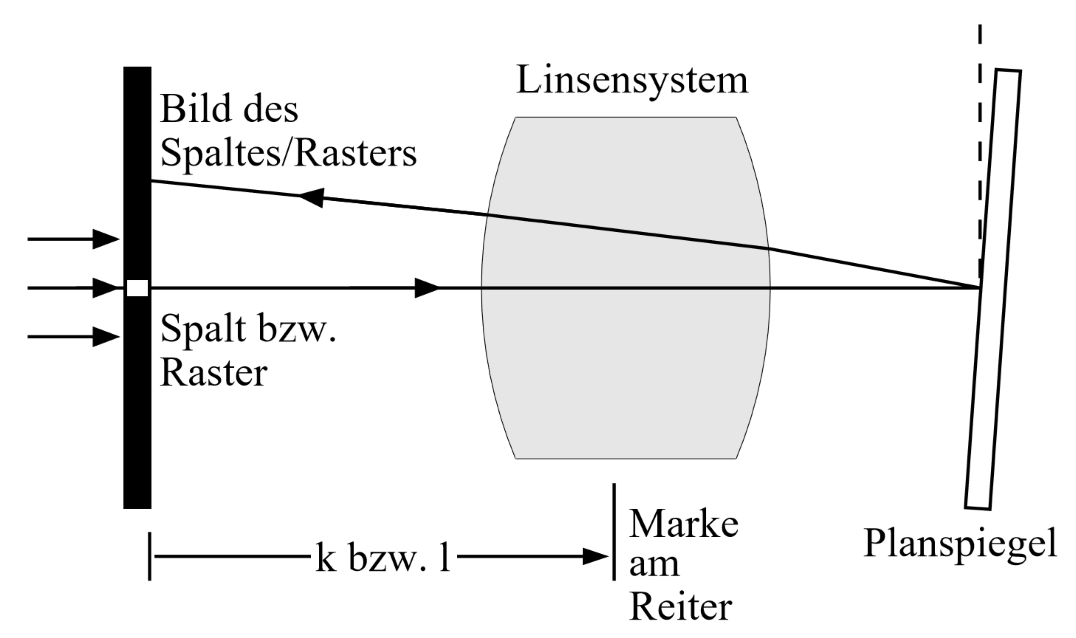
\includegraphics[width=0.8\textwidth]{Autokollimation_abb.png}
        \caption{Versuchsaufbau zum Autokollimationsverfahren}   % Quelle Fehlt
        \label{fig:autoKollAbb}
    \end{figure}

    \subsection{Besselmethode}
    Bei der Besselmethode wird die zu untersuchende Linse zwischen Blende und Schirm wie in Abbildung \ref{fig:BesselAbb} veranschaulicht gestellt.
    Es gibt nun zwei Positionen, bei denen ein scharrfes Bild auf dem Schirm entsteht. Aus der Differenz dieser Positionen und dem Abstand von Blende und Linse folgt nun für den Brechungsindex und den Hauptebenenabstand:
    \begin{align}
    
        f' = \frac{1}{4} \cdot [(e-h)-\frac{d^2}{e-h}] \label{eq:besselBrech1}\\
        f = \frac{1}{4} \cdot [\frac{d^2}{e-h}-(e-h)] \label{eq:besselBrech2}
            
    \end{align}

    Kombiniert man nun Autokollimationsverfahren und die Besselmethode, so lassen sich beide Größen, Brechungsindex und Hauptebenenabstand, berechen:
    
    \begin{align}
    
        f' = \frac{1}{2} \sqrt{(e-k-l)^2-d^2}\\
        h = k+l- \sqrt{(e-k-l)^2-d^2}
            
    \end{align}
    

    \begin{figure}
        \centering
        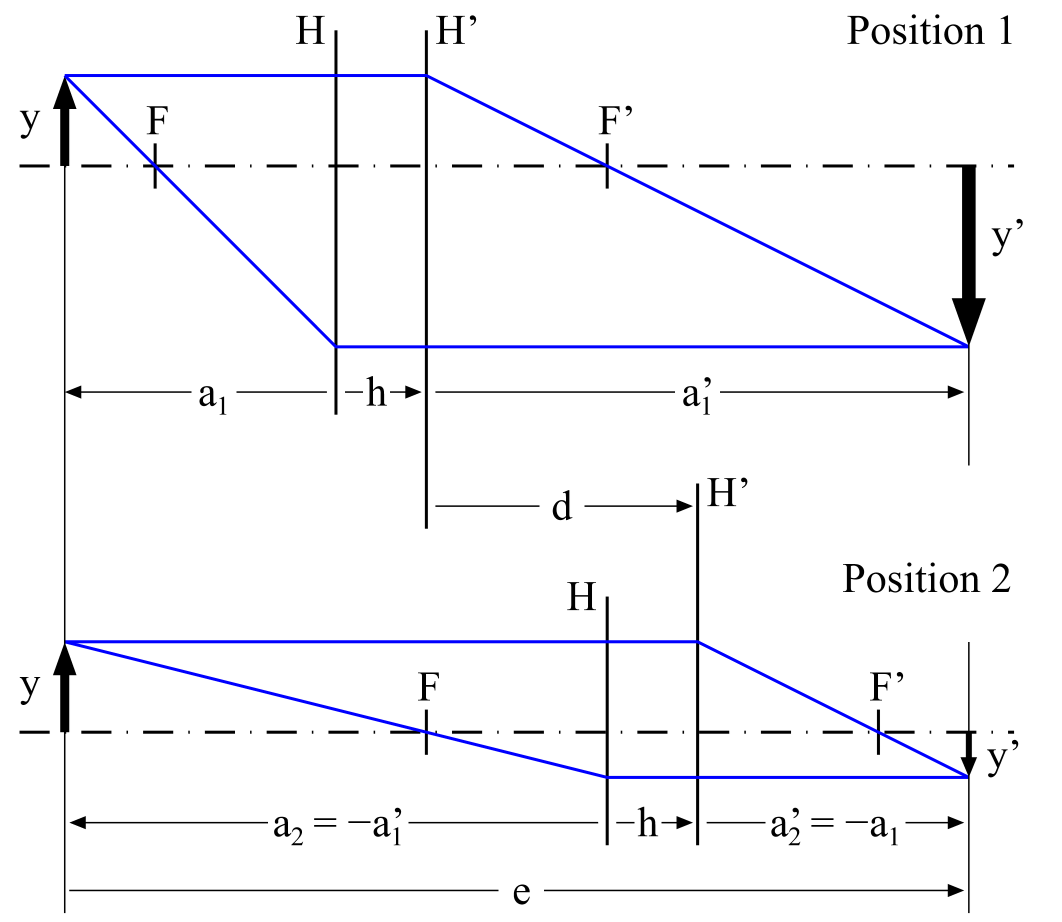
\includegraphics[width=0.8\textwidth]{Bessel_Abb.png}
        \caption{schematischer Versuchsaufbau der Besselmethode}   % Quelle Fehlt
        \label{fig:BesselAbb}
    \end{figure}

    \subsection{Abbemethode}

    \section{Ergebnisse}
    \subsection{Vorhandene Linsen}
    Bei dem Versuch standen uns verschiedene Linsen zur Verfügung mit unterschiedlichen Brecheigenschaften wie in Tabelle \ref{tab:Brecheig} zu sehen ist.
    
    \begin{table}
        \centering
        \begin{tabular}{c|c}
            
            Linse & Brecheigenschaften \\ \hline
            A & Sammellinse \\ \hline
            B & Sammellinse \\ \hline
            C & Sammellinse \\ \hline
            E & Sammellinse \\ \hline
            G & Streulinse \\ \hline

            
        \end{tabular}
        \caption{Brecheigenschaften der vorhanden Linsen}
        \label{tab:Brecheig}
    \end{table}
    
    \subsection{Autokollimation bei dünnen Linsen}
    In diesem Versuchsteil wurden die dünnen Linsen B und G auf ihren Brechungsindex untersucht mit dem Autokollimationsverfahren.
    Dazu wurde dieses fünf mal angewendet und der Mittelwert berechnet. Die Fehler ergeben sich mithilfe der student-Verteilung und gaußscher Fehlerfortpflanzung.
    Aus den Längen $l$ und $k$ lässt sich mit der Formel \ref{eq:autokollBrech} (mit Hauptebene $h=0$) der Brechungsindex berechnen. Die Ergebnisse sind in Tabelle \ref{tab:BGAutokoll} dargestellt.


    \begin{table}
        \centering
        \begin{tabular}{c|c|c|c}
            
            Linse & $l$ & $k$ & Brechungsindex $f$ \\ \hline
            B & 10,06(10) $\si{\centi\meter}$& 9,91(10) $\si{\centi\meter}$& 9,98(07) $\si{\centi\meter}$\\ \hline
            G & 7,44(10) $\si{\centi\meter}$& 7,57(10) $\si{\centi\meter}$&  7,50(07) $\si{\centi\meter}$\\ \hline

            
        \end{tabular}
        \caption{Ergebnisse Brechungsindex von Linse B und G mit dem Autokollimationsverfahren}
        \label{tab:BGAutokoll}
    \end{table}
    
    \subsection{Besselverfahren be dünnen Linsen}
    Nun wird der Brechungsindex erneut der Linsen B und G mit dem Besselverfahren bestimmt. Auch bei diesem Versuchteil wurden die Messungen fünf mal wiederholt und anschliesend der Mittelwert der Differenz $d$ gebildet.
    Unter der Annahme, dass bei einer dünnen Linse die Hauptebene $h=0$ ist kann Der Brechungsindex mit Formel \ref{eq:besselBrech1} bzw. \ref{eq:besselBrech2} berechnet werden (siehe Tabelle \ref{tab:BGBessel}).

    \begin{table}
        \centering
        \begin{tabular}{c|c|c|c}
            
            Linse & Differenz $d$ & Länge $e$ & Brechungsindex $f$ \\ \hline
            B & 38,29(10) $\si{\centi\meter}$& 63,10(29) $\si{\centi\meter}$& 9,97(10) $\si{\centi\meter}$\\ \hline
            G & 21,77(10) $\si{\centi\meter}$& 41,40(29) $\si{\centi\meter}$&  7,49(10) $\si{\centi\meter}$\\ \hline

            
        \end{tabular}
        \caption{Ergebnisse Brechungsindex von Linse B und G mit dem Besselverfahren}
        \label{tab:BGBessel}
    \end{table}
     Sowohl das Autokollimationsverfahren als auch das Besselverfahren ergeben zueinander konsistente Werte. Jdeoch ist das Besselverfahren etwas ungenauer.
    

    \bibliographystyle{plain}
    \bibliography{literature}

\end{document}